\documentclass[14pt, a4paper]{article}
\usepackage[T2A]{fontenc}
\usepackage[utf8]{inputenc}
\usepackage[russian]{babel}
\usepackage[left=3cm, right=1.5cm, top=2cm, bottom=2cm]{geometry}
\usepackage{indentfirst}
\usepackage{microtype}
\usepackage{array}
\usepackage{xcolor}
% \usepackage{times}
\usepackage{tempora}
\usepackage{ulem}
\usepackage{setspace}
\usepackage{amsmath}
\usepackage{booktabs}
\usepackage{graphicx}
\usepackage{float}
\usepackage{listings}
\graphicspath{{reports/figures/}{figures/}}
\lstset{basicstyle=\ttfamily\small, breaklines=true, columns=fullflexible, frame=single, keepspaces=true}
\pagestyle{empty}

\makeatletter
\renewcommand\section{\@startsection {section}{1}{\parindent}%
  {-3.5ex \@plus -1ex \@minus -.2ex}%
  {0.5ex}%
  {\normalfont\Large\bfseries}}
\renewcommand\tableofcontents{%
  \begin{center}\Large\bfseries\contentsname\end{center}%
  \@starttoc{toc}%
}
\renewcommand*\l@section{\@dottedtocline{1}{0em}{1.5em}}
\makeatother

\begin{document}
\onehalfspacing

\begin{center}
    \textbf{ФЕДЕРАЛЬНОЕ ГОСУДАРСТВЕННОЕ АВТОНОМНОЕ ОБРАЗОВАТЕЛЬНОЕ} \\
    \textbf{УЧРЕЖДЕНИЕ ВЫСШЕГО ОБРАЗОВАНИЯ} \\
    \textbf{«МОСКОВСКИЙ АВИАЦИОННЫЙ ИНСТИТУТ} \\
    \textbf{(НАЦИОНАЛЬНЫЙ ИССЛЕДОВАТЕЛЬСКИЙ УНИВЕРСИТЕТ)»}
\end{center}

\begin{center}
    \bfseries Институт №8 «Компьютерные науки и \\
    \bfseries прикладная математика» \\
    \bfseries Кафедра 806 «Вычислительная математика \\
    \bfseries и программирование»
\end{center}

\vspace{3cm}

\begin{center}
    \Large\bfseries Отчет \\
    \vspace{0.5cm}
    \mdseries по лабораторной работе №3.4
\end{center}

\vfill

\noindent
\hfill
\begin{tabular}{ll}
Группа:       & М8О-307Б-21 \\
Студент:      & М. С. Ивченко \\
Преподаватель:& доц. В. В. Киндинова \\
Оценка:       & \underline{\makebox[3cm][c]{}} \\ [0.2cm]
Дата:         & \underline{\makebox[3cm][c]{}}
\end{tabular}

\vfill

\begin{center}
    Москва \\
    2026
\end{center}

\newpage

\setcounter{tocdepth}{2}
\tableofcontents
\newpage

\section*{Тема}
\addcontentsline{toc}{section}{Тема}
Цель данной лабораторной работы -- освоить численное дифференцирование функций, заданных таблицей значений. Работа показывает, как по соседним узлам сетки можно приближенно вычислять первую и вторую производные в заданной точке.

\section*{Задание}
\addcontentsline{toc}{section}{Задание}
Вычислить первую и вторую производную от таблично заданной функции $y_i = f(x_i)$, $i = 0, 1, 2, 3, 4$ в точке $x = X^*$.

\section*{Теория}
\addcontentsline{toc}{section}{Теория}
Численное дифференцирование применяется, когда функция задана таблицей, а аналитическая формула неизвестна или неудобна. Производная заменяется разностными отношениями, построенными по соседним значениям функции. На равномерной или неравномерной сетке первая грубая оценка наклона на отрезке имеет вид
\[
    f'(x_i)\approx\frac{y_{i+1}-y_i}{x_{i+1}-x_i}
\]
или аналогично слева от точки. Такая формула имеет первый порядок точности и фактически дает наклон секущей, а не касательной.

Более точные формулы удобно получать через интерполяционный многочлен. Если взять три соседних узла и построить по ним квадратичный многочлен Ньютона, то его производная в точке $x$ дает формулу второго порядка:
\[
    f'(x)\approx f[x_i,x_{i+1}]+
    \left(f[x_{i+1},x_{i+2}]-f[x_i,x_{i+1}]\right)
    \frac{2x-x_i-x_{i+1}}{x_{i+2}-x_i}.
\]
Здесь $f[x_i,x_{i+1}]$ -- первая разделенная разность. Вторая производная вычисляется по изменению первых разностей:
\[
    f''(x)\approx 2\frac{f[x_i,x_{i+1}]-f[x_{i-1},x_i]}{x_{i+1}-x_{i-1}}.
\]
На практике нужно выбирать такие соседние узлы, чтобы точка $X^*$ лежала внутри соответствующего интервала. Численное дифференцирование чувствительно к ошибкам исходных данных: если табличные значения содержат шум, производные могут иметь заметно большую относительную ошибку, чем сами значения функции.

\begin{lstlisting}[language=Python]
f1 = (y[i + 1] - y[i]) / h1
f2 = (y[i + 2] - y[i + 1]) / h2
first = f1 + (f2 - f1) / (x[i + 2] - x[i]) * (2*x0 - x[i] - x[i+1])
second = 2 * (f2 - f1) / (x[i + 2] - x[i])
\end{lstlisting}

\section*{Ход лабораторной работы}
\addcontentsline{toc}{section}{Ход лабораторной работы}
Для точки $X^*=1.0$ задана таблица
\[
\begin{array}{c|ccccc}
x_i&0&0.5&1.0&1.5&2.0\\\hline
y_i&1.0000&1.3776&1.5403&1.5707&1.5839
\end{array}
\]
Получены значения:
\begin{table}[H]
\centering
\begin{tabular}{lr}
\toprule
Величина & Значение\\
\midrule
Левосторонняя $y'(1.0)$ & 0.3254\\
Правосторонняя $y'(1.0)$ & 0.0608\\
$y'(1.0)$ второго порядка точности & 0.0780\\
$y''(1.0)$ & -0.0688\\
\bottomrule
\end{tabular}
\caption{Результаты численного дифференцирования.}
\end{table}

\begin{figure}[H]
    \centering
    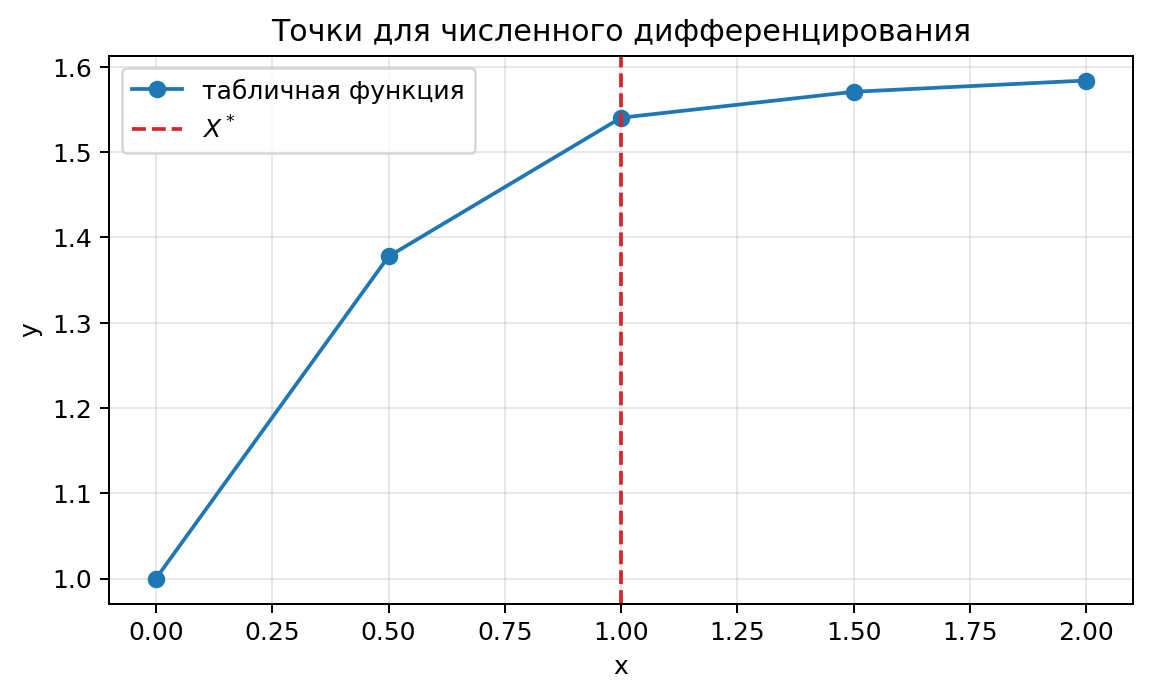
\includegraphics[width=0.86\textwidth]{lab3_4_derivatives.png}
    \caption{Табличные точки, использованные для вычисления производных в $X^*=1.0$.}
\end{figure}

\section*{Выводы}
\addcontentsline{toc}{section}{Выводы}
Односторонние оценки первой производной заметно отличаются, что указывает на кривизну табличной функции около $x=1$. Формула второго порядка использует соседние интервалы и дает более сглаженную оценку производной.

\end{document}
